\documentclass[a4paper,12pt]{article}
\usepackage{fullpage}
\usepackage{algorithm}
\usepackage{graphicx}
\usepackage{longtable}

\begin{document}
\begin{titlepage}
\noindent
\large\textbf{Deliverable 1} \hfill \textbf{Nayana Raj Cheluvaraju} \\
\normalsize SOEN 6011 \hfill \textbf{40071318} \\
Prof. P.Kamthan \hfill Due Date: 19/07/2019 \\
\hspace*{\fill}\texttt{{https://github.com/}{nayanarajc/SOEN\_6011}}\\

    \begin{center}
        \large\textbf{F10:$\sigma$}
    \end{center}

\section{Problem 1 -Description}
This symbol notifies standard deviation(SD), it is a method that measures extent of variation or separation of data values. The symbol $\sigma$  is taken from Greek letter sigma. If the value of standard deviation is low it indicates data points are close to the mean, while higher value indicates wider range of values.The values that goes into the function is called as domain, all possible outcome of function is co-domain and actual output from system is called Range. Things required to calculate standard deviation are mean and variance. Mean is calculated by summing up all values and dividing it by total number of values and variance is calculated by taking difference of each, squaring it and then averaging the results. Calculator will compute population and sample standard deviation.\newline
The Range for standard deviation is between negative infinity to positive infinity\newline
\textbf{Properties of Standard Deviation}\newline
1.	Measures spread-out numbers.\newline
2.	It is expressed in same unit as data.\newline
3.	Used to measure statistical results such as margin of errors.\newline
4.	Using standard deviation, we can calculate normal, extra-large and extra small values.
\newline
\newline
\textbf{Population Standard Deviation}
\newline
This is used when an entire population can be measured, and where every member of a population can be sampled. The following is the equation:
\begin{center}
\begin{math}
\sigma=\sqrt{\frac{1}{N}\Sigma_{i=1}^{N}(x_{i}-\mu)^2}
\end{math}
\end{center}
Where xi is one individual value,$mu$ is the mean/expected value, N is the total number of values
\newline
\newline
\textbf{Sample Standard Deviation}
\newline
In this it is not possible to sample every member within a population, so above equation must be modified such that the deviation can be measured through random samples of the population. 
\begin{center}
\begin{math}
s= \sqrt{\frac{1}{N-1}\Sigma_{i=1}^{N}(x_{i}-\bar{x})^2}
\end{math}
\end{center}
Where xi is one sample value,$\bar{x}$ is the sample mean and N is number of sample value.

\section{Problem 2 -Requirements And Assumptions}
\subsection{Functional Requirements}
1: Low priority , 5:High Priority
\subsubsection{Input Requirement}
When the user enters zero input/input=null, the function shall pop out an error stating "Input cannot be Null". As number divided by zero leads to infinity. (length !=0)\newline
Priority of this requirement: 5
\subsubsection{Length Requirement}
When the user enters less than two inputs, the function shall display error message "Enter more than one input". This is because minimum length required to calculate standard deviation is 2.(min length=2)\newline
Priority of this requirement: 5
\subsubsection{Multiple inputs}
User shall be able to enter 'n' inputs from the console provided by function.There is no limit for inputs. Function has to handle inputs.\newline
Priority of this requirement: 3
\subsubsection{Handling real numbers}
As user enters real numbers, the function shall be able to accept, process it and output's as real numbers.\newline
Priority of this requirement: 3
\subsubsection{Calculate Mean}
When calculating standard deviation function, the function shall automatically call mean and retrieve result without notice to user. \newline
Priority of this requirement: 4
\subsubsection{Calculate variance}
When calculating standard deviation function, the function shall calculate variance explicitly or within the function and retrieve result without getting to user notice. \newline
Priority of this requirement: 4
\subsubsection{Display Output}
User shall be able to see only final output of function which is Standard deviation value, and output will be displayed on console. User shall not have any problem while viewing output. \newline
Priority of this requirement: 5
\subsection{Non-Functional Requirements}
\subsubsection{Performance}
It is analysed on how the function responds to given input provided at certain time. 
\subsubsection{Correctness}
Correctness of the function is measurable by checking input-output behaviour.The generated output is verified by comparing results computed manually.
\subsubsection{Consistency}
The consistency of the function remains same throughout all calculators, as math definition for standard deviation is unchangeable. And consistency of output for all input also remains same.
\subsubsection{Accessibility}
Defines how easily the function is accessible by all kinds of stakeholders, in different platforms and with integration of hardware.
\subsubsection{Usability}
The function is easily usable by all stakeholders and also learn-able to achieve specific needs.

\subsection{Constraints}
1.	Interfaces for calculating standard has already been defined and is not bounded to change.\newline
2.	Some calculators are region specific.\newline
3.  Mode for selecting standard deviation may vary from different calculators.\newline
4.  Users from non-mathematical background will have difficulties in accessing function through calculator.

\subsection{Assumptions}
1.	All inputs provided by users are real numbers.\newline
2.	Inputs are of population standard deviation.\newline
3.	Users will be familiar with accessing functions in calculator.\newline
4.	All calculators that supports Math and Statistics contains standard deviation function.\newline 
5.	Value of standard deviation directly proportional to data points or mean value.

\section{Problem 3 - Pseudocode And Algorithm}
\newpage
\begin{algorithm}
\caption{Squareroot(number)- common for both Iterative and Recursive}
begin: \\
1. SET Sqrt=number/2\\
2. $\hspace{2em}$ Do\\
3. $\hspace{3em}$ temp=sqrt\\
4. $\hspace{3em}$ Add temp value with (number/temp) and divide whole by 2\\
5. $\hspace{3em}$ CONTINUE WHILE ((temp - result) != 0)\\
6. RETURN result\\
end
\end{algorithm}
\subsection{Using Iterative Approach}
\textbf{\textit{Advantages:}}\newline
1. Easier to understand.\newline
2. Saves memory.\newline
3. Iterative approach can enhance time and space requirement.\newline
4. Fast in execution.\newline
\newline
\textbf{\textit{Disadvantages:}}\newline
1. The iterative repeatedly dynamically allocate or resize memory blocks.\newline
2. Time consuming to Recursive approach.\newline
3. Contains duplicate code.\newline
4. Iteration makes the code longer.\newline
\begin{algorithm}
\caption{calculateMean(array) And CalculateStandardDeviation (array[])}
\label{Algorithm 1:}
begin: \\
1. SET Counter=0\\
2. $\hspace{2em}$FOR Counter$<$length THEN\\
3. $\hspace{3em}$ Add all values\\
4. $\hspace{3em}$INCREMENT Counter by 1 \\
5. mean= Total/length \\
6. RETURN mean\\
end\newline
begin: \\
1. COMPUTE Mean(array)\\
2. SET Counter=0\\
4. $\hspace{2em}$FOR Counter$<$length THEN\\
5. $\hspace{3em}$ Subtract each value from Mean\\
6. $\hspace{3em}$ Square the subtracted value and keep adding     with previous squared values\\
7. $\hspace{3em}$INCREMENT Counter by 1 \\
9. result= calculatedsum/length \\
10. COMPUTE Squareroot(result)\\
11. RETURN computed result \\
12.REPEAT the algorithm for new value  \\
end
\end{algorithm}
\newpage
\subsection{Using Recursive Algorithm}  
\textbf{\textit{Advantages:}}\newline
1. Allows to allocate additional automatic objects at each function call.\newline
2. Faster compared to Iterative approach.\newline 
3. Makes the problem more elegant.\newline
4. Reduces Time complexity of a program.\newline
\newline
\textbf{\textit{Disadvantages:}}\newline
1. Makes the execution slower.\newline
2. Takes up more of stack storage.\newline
3. Difficult to understand and trace.\newline
\begin{algorithm}
\caption{calcStd(List)}
begin:\\
calcAvg(List)\newline
1. COMPUTE calcSum(list,0)\\
2. Divide sum by size of list\\
3. RETURN result\\
end\newline
begin:\\
calcSum(List, i)\newline
1. IF i$<$ size of list THEN\\
2. $\hspace{2em}$ Add each element(i) with its next element(calcSum(list,i+1))\\
3. $\hspace{2em}$ RETURN result\\
4. ELSE\\
5. $\hspace{2em}$ RETURN 0\\
end\newline
begin:\\
calcpow(List,avg,i)\newline
1. IF i$<$ size THEN\\
2. $\hspace{2em}$ Subtract each value with Avg \\
3. $\hspace{2em}$ Square the result\\
4.  $\hspace{2em}$ RETURN square\\
5. ELSE\\
6. $\hspace{2em}$RETURN 0\\
end\newline
begin:\\
sumSquareDiffs(List,avg,i)\newline
1. IF i$<$ size THEN\\
2. $\hspace{2em}$ COMPUTE calcpow(List,avg,i) \\
3. $\hspace{2em}$ keep adding result of each element\\
4. ELSE\\
5. $\hspace{2em}$ RETURN 0\\
end\newline
begin:\\
calcStd(List)\newline
1. COMPUTE calcAvg(List)\\
2. COMPUTE sumSquareDiffs(List,avg,i) taking avg value from step2\\
3. COMPUTE Squareroot(sum) take sum value from step3 and Squareroot() from algorithm 1\\
4. RETURN result\\
end\newline
\end{algorithm}
\newpage

%%%%%%%%%%%%%%%%%%% DELIVERABLE 2 %%%%%%%%%%%%%%%%%%%%
\section{Changes from D1 to D2}
Added Extra Functional Requirements\\
2.1.8 Entering consecutive repetition of same number.\\
2.1.9 Showing difference between  sample and population SD

\section{Problem 4} 
\subsection{Debuggers}
Debugging is the common process of identifying and removing bugs, errors or abnormalities from programs. It is a required skill for all Java developers, because it helps to find subtle bug that are not visible during code reviews or that only happens when a specific condition occurs. The Eclipse Java IDE provides many debugging tools and views grouped in the Debug Perspective to help the you as a developer debug effectively and efficiently.
There are many improvements in Eclipse Java Development Tools(JDT) included from Eclipse Oxygen on-wards. \newline
The debuggers used for this project are:\newline
1. Command Line Debuggers\newline
2. IDE Debuggers\newline
The Images for 1 and 2 types have been attached in \textit{Appendix section} at the end.\newline
\textbf{\textit{Challenges faced}}: Also tried installing Eclipse-Mirur visual Debugger which gives one dimensional view of the debugging result but after installing it was not working.\\ 
\newline
\textbf{1.Java debugger(JDB)}: is a tool used to debug java program in command Line. It implements the java platform debugger architecture. It helps in detecting and fixing bugs in program with help of java debug interface.\newline
\textbf{\textit{Advantages}}\newline
1. Allows breakpoints, an explicit way of stop or pause application.\newline
2. Enables stepping process, its a debugger feature that lets you to execute line by line.\newline
3. It also throws uncaught exception with its cause.\newline
\textbf{\textit{Disadvantages}}\newline
1. It is slow compared to IDE debuggers.\newline
2. Complete visual flow of debugging process in not available.\newline
3. Not user friendly, as compared to IDE.\newline
\newline
\newline
\textbf{2. IDE Debugger}: These are built in debugging tool with eclipse for java. Eclipse allows to begin java program in debug mode. It has all features that consists in JDB and also allows extra features such as watchpoint-is a break-point set on field. Exception breakpoints, method breakpoints, step filter, hit count, remote debugging and drop to frame- allows to select level of frame.\newline  
\newline
\textbf{\textit{Advantages}}\newline
1. Debug perspective offers additional view.\newline
2. Stepping commands(stop,start,resume) are easily accessible, as its built as buttons. \newline
3. Enables creation of own debugger.\newline
4. Consumes less time and effort for organizing resource, provides shortcuts and track mistakes.\newline
\textbf{\textit{Disadvantages}}\newline
1. As high end desktop application, these cannot run on production machine. \newline
2. Possibility of remote debugging will be ruled out for complex environments. \newline
3. Learning curve- maximizing benefits will require lot of time and patience.\newline
4. Will not fix bad code,coding standard or performance problems.

\subsection{Quality Attributes}
Program is set such that it satisfies quality as expected by user.\\
1. \textit{\textbf{Correctness}}: \\Is satisfied by verifying the results of standard deviation given from the program. This is achieved by comparing with manual calculation or calculating from online tool.Unit testing is also written such that it measures correctness.\\
2. \textit{\textbf{Efficiency}}:\\ Measured by time taken to run the program and display the output. Here the program is utilizing minimum amount of resources as all functions are implemented and in same class memory required is also less.All these results in more efficiency.\\
3. \textit{\textbf{Maintainable}}: \\As the program is structured using coding standards it is easily maintainable and flexible to future changes. User can easily follow the program. GUI is also maintainable and extendable as its structured and simple to handle.\\
4. \textit{\textbf{Robust}}: \\safety measures are taken to cope up with the errors during execution by incorporating \textit{try and catch block} with letting user know from proper message popup and also GUI buttons are made clear so its less prone to errors.\\
5. \textit{\textbf{Usable}}: Program is divided into different function so that each function can be executed individually and can be reused in other programs easily.Usage is also not restricted to once.\\
\textbf{\textit{Challenges faced}}:\\
1. Tried installing Ecipse-Jdepend and Eclipse-JDeodorant for estimating quality attributes, but after installation had hard time finding them.\\
2. Lack of explanation in documentation and as they are huge required information is hard to find.

\subsection{Quality Checker}
Quality of the program or source code is verified by exposing code under checking tools. For this project there are two tools used: 1.Checkstyle and  2.PMD . 
\subsubsection{Checkstyle}
The source code standard Checkstyle checks are applicable to java program and requires no external libraries. Checkstyle provides many checks such as naming,location of annotation,nested blocks,constant names,empty block, illegal token, type, javadoc, tags, method name, count and much more. \newline
\newline
\textbf{\textit{Advantages}}\newline
1. Portability between IDE's - If we want to use visual studio or my team member is using other IDEs still it exhibits consistency.\\
2. Easy to use as its integrated as an external tool designed which can be hooked into the code easily. Whereas in Eclipse styler we need to locate the plugin to do same task.\\
3. Ability of creating own rules- checkstyle provide user to add his own custom rules.\newline
\newline
\textbf{\textit{Disadvantages}}\newline
1. Errors are fixed manually, there is no automatic fix.\\
2. The symbol used to display errors are same as eclipse warnings which leads to confusion.\\
3. Few errors are not understandable.\\
4. It just mentions error does not say in which part user should keep doing trial and error to fix it.\\
\subsubsection{Eclipse-PMD}
PMD is a static source code analyzer which finds programming flaws such as unused variables, empty catch blocks, unnecessary object creation, and so forth. Once installed, every time while saving work it also checks for potential problems like possible bugs, duplicate, dead or complicated code.Eclipse PMD offers quick fixes that automatically fixes the problem which can be of single fix or all occurrences in entire code. It categorizes errors based on severity. This is bit advanced tool compared to checkstyle with having more features as its packed with 149 rules.\\
\newline
\textbf{\textit{Advantages}}\newline
1. Scalability is high as tool runs well for very large source code.\\ 
2. Comply with coding standards and delivery quality code. \\
3. Used by teams to change the nature of code reviews.\\
4. Reduces software maintenance cost. As its open source tool and time spent is less.\newline
5.PMD can also be customized to meet organization coding standard and quality.\\
\newline
\textbf{\textit{Disadvantages}}\newline
1. Even this intend user to correct errors manually.Cannot find runtime issues\\
2. As PMD comes by rules there is certain time clash of rules when used with other tools.\\
3. The documentation guide is overwhelming to users, it does not give examples of output or how to best run PMD. \\
4. Creating new rule requires understanding of Abstract syntax tree(AST).\\
\newline
Images for both checkstyle and PMD are added in Appendix section.

\section{Problem 6- Unit Testing}
\subsection{Traceability Record}
The below table shows the mapping of test case with requirements.
\begin{center}
\begin{longtable}{|l|l|l|}
\caption{Table shows Traceability Record.} \label{tab:long} \\
\hline \multicolumn{1}{|c|}{\textbf{Test Case #}} & \multicolumn{1}{c|}{\textbf{Test Case Name}} & \multicolumn{1}{c|}{\textbf{Related Requirement(s)}} \\ \hline 
\endfirsthead

\multicolumn{3}{c}%
{{\bfseries \tablename\ \thetable{} -- continued from previous page}} \\
\hline \multicolumn{1}{|c|}{\textbf{Test Case #}} & \multicolumn{1}{c|}{\textbf{Test Case Name}} & \multicolumn{1}{c|}{\textbf{Related Requirement(s)}} \\ \hline 
\endhead

\hline \multicolumn{3}{|r|}{{Continued on next page}} \\ \hline
\endfoot

\hline \hline
\endlastfoot

1 & CalculateMeanTest & 2.1.5 \\
2 & CalculateStdDevTest & 2.1.6 \\
3 & CalculateStdDevTest & 2.1.4 \\
4 & CalculateStdDevTest & 2.1.3 \\
5 & Graphical user Interface & 2.1.2 \\
6 & Graphical user Interface & 2.1.1 \\
7 & Graphical user Interface & 2.1.7 \\
8 & CalculateStdDevTest & 2.1.8 \\
9 & CalculateStdDevTest & 2.1.9 \\
\end{longtable}
\end{center}
The diagram below shows the results of testing. For testing Junit framework is used and test results have been tracked.\\
\newline
Figure1: Shows the results of JUnit \\
\newline
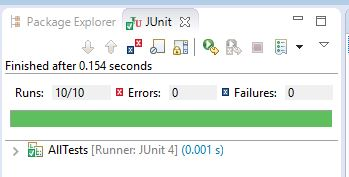
\includegraphics[width=9.0cm]{Testing result.JPG}\\
\newline
Below diagram shows the coverage of testing. Test results for GUI are not written as all the error messages are visible in the interface.\\
\newline
Figure2: Shows the test coverage for StandardDeviation.java file \\
\newline
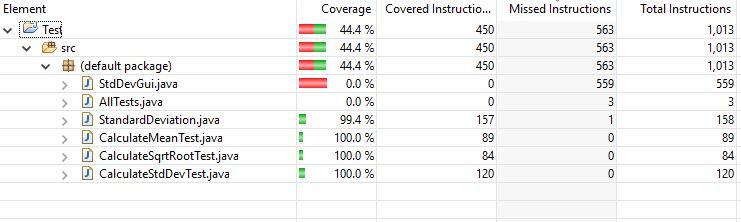
\includegraphics[width=9.0cm]{Coverage.JPG}\\
\newline
This project have been implemented and interfaced using graphical(GUI) user interface. For GUI implementation Java swings have been used. Below diagram shows the snippet of Interface. 
Figure3: Shows the Graphical User Interface(GUI) \\
\newline
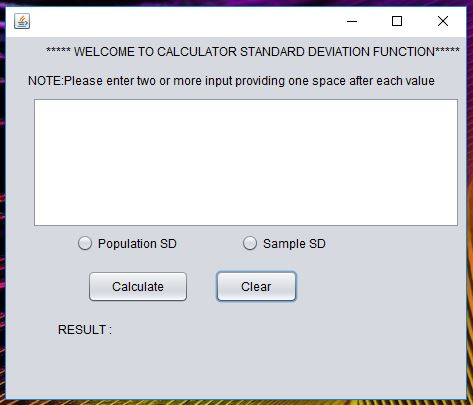
\includegraphics[width=9.0cm]{GUI.JPG}\\
\newline





\section{Appendix}
Figure1: Command-line Debugger used for F10 function \\
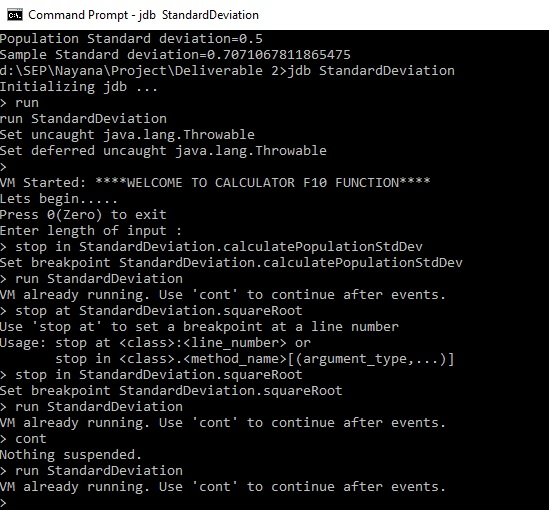
\includegraphics[width=9.0cm]{JDBDebugger.jpg}\\
\newline
Figure2: Eclipse IDE-Debugger\\
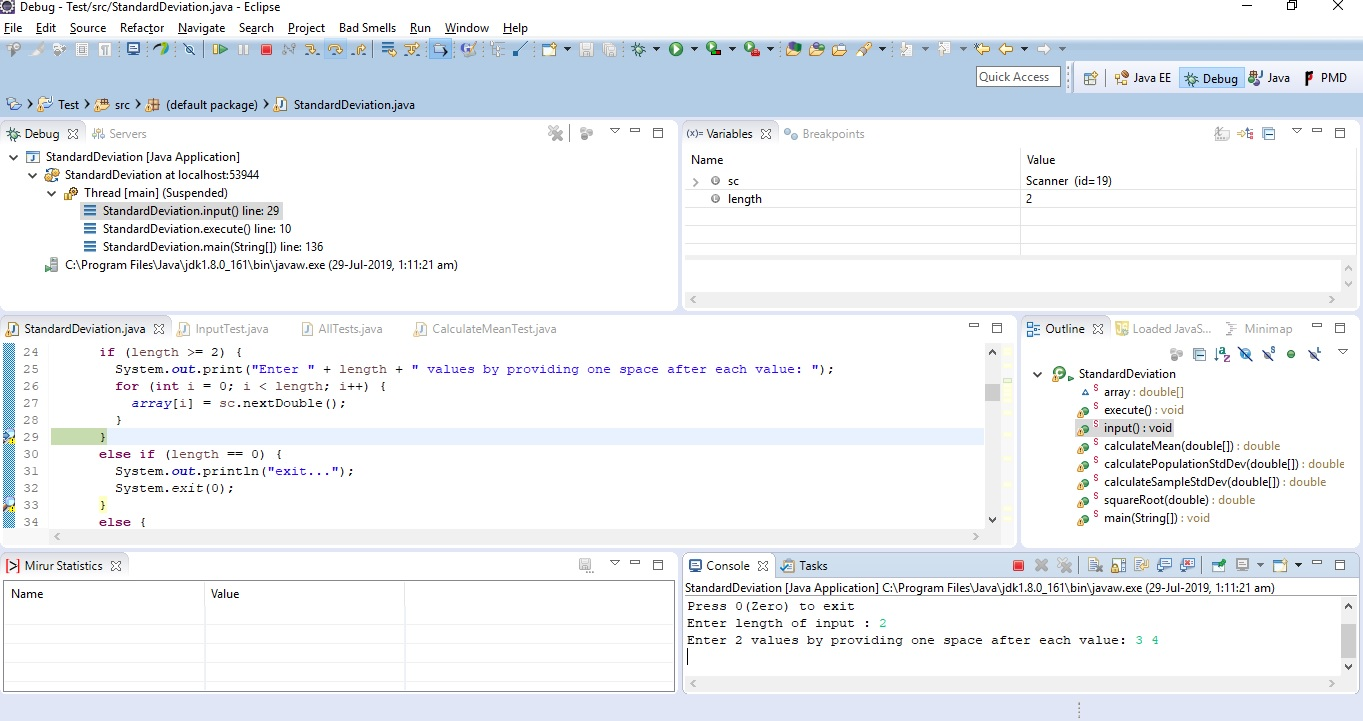
\includegraphics[width=10.0cm]{IDE-SC.jpg}\\
\newline
Figure3: Eclipse-CheckStyle\\
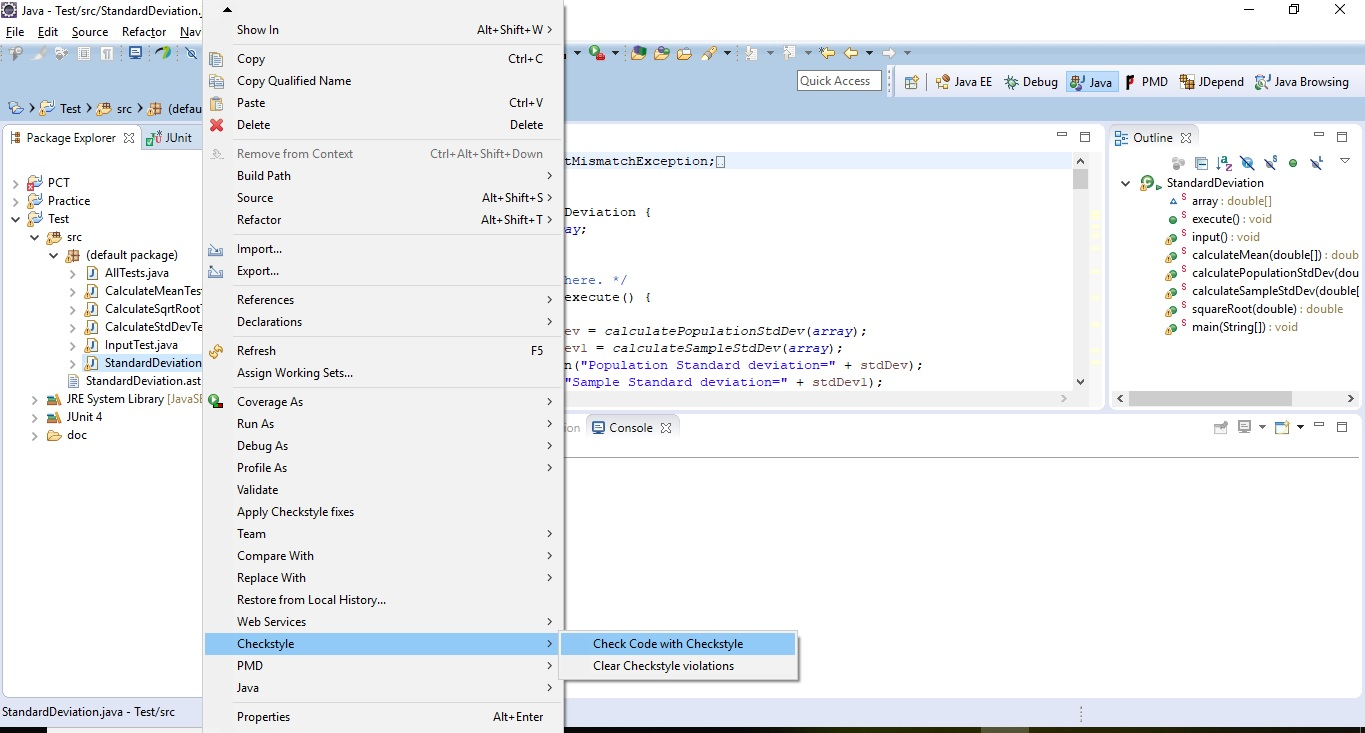
\includegraphics[width=10.0cm]{Checkstyle.jpg}\\
\newline
Figure4: Eclipse-PMD quality checker\\
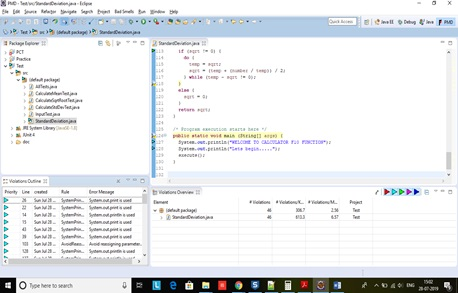
\includegraphics[width=10.0cm]{PMD-SC.jpg}\\

\section{Reference}
\bibliographystyle{plain}
\bibliography{Reference}

https://ieeexplore.ieee.org/stamp/stamp.jsp\newline
https://www.calculator.net/standard-deviation-calculator.html\newline
https://www.mathsisfun.com/data/\newline
https://tex.stackexchange.com/questions/88388/how-to-have-the-title-at-the-top-of-a-latex-document\newline
https://tex.stackexchange.com/questions/456051/standard-deviation\newline
https://www.reqview.com/doc/iso-iec-ieee-29148-srs-example.html\newline
https://users.csc.calpoly.edu/~jdalbey/SWE/pdl_std.html\newline
https://benpfaff.org/writings/clc/recursion-vs-iteration.html\newline
https://www.geeksforgeeks.org/how-to-write-a-pseudo-code/\newline
https://stackoverflow.com/questions/29022672/calculating-standard-deviation-of-array-recursively\newline
https://tutorialspoint.com/jdb/\newline
https://docs.oracle.com/javase/7/docs/technotes/tools/windows/jdb.html\newline
https://dzone.com/articles/definitive-list-7-java#IDE%20debuggers\newline
https://stackoverflow.com/questions/13644624/advantage-of-using-checkstyle-rather-than-using-eclipse-built-in-code-formatter\newline
https://marketplace.eclipse.org/content/eclipse-pmd\\
https://www.eclipsezone.com//articles/pmd/\\
http://www.cs.cmu.edu/~aldrich/courses/654/tools/hsu-pmd-07.pdf\\


\end{titlepage}
\end{document}
